\chapter{Results and analysis}
\label{ch5}
In this chapter, the results of the different methods will be reported. \\

\noindent The results are run on two main machines: Google Colab (\cite{gcolab}) for the forecasting part and my personal laptop for the controlling part.\\
Two systems are used for two main reasons: the possibility to run both forecasting and controlling tests at the same time and to reduce the training time (especially for the forecasting part) thanks to the powerful hardware from Google.\\
The laptop used is a Xiaomi Mi Laptop Air 13.3 (2017) with an Intel Core i5 6200U 2.30GHz CPU, a 8GB 1064MHz RAM and an NVIDIA GeForce 940MX 1023MB GPU.

\section{Forecast results}
\label{sec:5fr}
In this section, the results obtained when solving the aim \ref{aim2} are reported.\\

For the forecasting task, some evaluation metrics are used to test the performance of the \gls{ANN}. These metrics are: accuracy, recall, precision and F1-score. \\
During training, the F1-score on the validation set of the model is monitored, and the best weights configuration is stored. The score reported in the following tables, are obtained testing the model on the test set, with the most performing saved model. \\
It is worth mentioning that, at the time of this thesis development, the core TensorFlow library allows monitoring only the accuracy, recall, precision but not the F1-score; this can take to misleading, and it can lead to suboptimal results. For this reason, a custom monitor of the F1-score is developed.\\

In this thesis, three values of $h$ are used: 2, 4 and 16 corresponding to have the past information of the system of 30 minutes, 1 hour and 4 hours. For the $n$, only one value is used: 1, corresponding to a short planning time of 15 minutes ahead.\\

The three combinations are tested, and the results are reported as an average of 5 runs. The models are trained for 100 epochs on the training set, for each epoch the neural network is evaluated on the validation set and the best performing model is used to get the score on the testing set.\\
The batch size is 512. This is important since the dataset is unbalanced; in this way there is a high chance that each batch contains a decent amount of voltage problems to learn from.
% \begin{enumerate}[label=\roman*)]
\begin{itemize}
    \item Results of the first combination \ref{onlyV}:
    
    \begin{table}[H]
    \centering
    %\resizebox{\textwidth}{!}{%
    \begin{tabular}{|c|l|c|c|c|c|c|}
    \hline
    \textbf{h} &
      \textbf{Models} &
      \multicolumn{1}{l|}{\textbf{Accuracy}} &
      \multicolumn{1}{l|}{\textbf{Precision}} &
      \multicolumn{1}{l|}{\textbf{Recall}} &
      \multicolumn{1}{l|}{\textbf{F1-score}} &
      \multicolumn{1}{l|}{\textbf{Time (s)}} \\ \hline
    \multirow{3}{*}{\textbf{2}}  & \textbf{MLP} & 0.979 & 0.786 & 0.833 & 0.804                           & 73  \\ \cline{2-7} 
                        & \textbf{CNN} & 0.981 & 0.793 & 0.862 & 0.825                           & 67  \\ \cline{2-7} 
                        & \textbf{RNN} & 0.981 & 0.798 & 0.858 & \textbf{0.826} & 121 \\ \hline
    \multirow{3}{*}{\textbf{4}}  & \textbf{MLP} & 0.979 & 0.817 & 0.777 & 0.792                           & 74  \\ \cline{2-7} 
                        & \textbf{CNN} & 0.980 & 0.795 & 0.851 & 0.820                           & 70  \\ \cline{2-7} 
                        & \textbf{RNN} & 0.981 & 0.796 & 0.860 & \textbf{0.827} & 205 \\ \hline
    \multirow{3}{*}{\textbf{16}} & \textbf{MLP} & 0.978 & 0.800 & 0.797 & 0.796                           & 77  \\ \cline{2-7} 
                        & \textbf{CNN} & 0.798 & 0.798 & 0.822 & 0.810                           & 81  \\ \cline{2-7} 
                        & \textbf{RNN} & 0.980 & 0.786 & 0.866 & \textbf{0.823} & 441 \\ \hline
    \end{tabular}%
    %}
    \caption[Models' results using voltage information]{Results using as input the voltage information at each bus.}
    \label{tab:onlyV}
    \end{table}
    This task is the simplest case, since the goal is to predict the future of a particular quantity (voltage) given the past information of the same quantity.\\
    From table \ref{tab:onlyV}, It is possible to see that the \gls{RNN} model performs better than the other models, since usually \gls{RNN} handles better time series data. Moreover, it would be expected that the more data the \glspl{ANN} receive as input (value of h), the higher the score it gets, but for this task, results look like are independent of the value of $h$.
    
    \item Results of the second combination     \ref{LpqandGp}:
    
   \begin{table}[H]
    \centering
    % \resizebox{\textwidth}{!}{%
    \begin{tabular}{|c|l|c|c|c|c|c|}
    \hline
    \textbf{h} &
      \textbf{Models} &
      \multicolumn{1}{l|}{\textbf{Accuracy}} &
      \multicolumn{1}{l|}{\textbf{Precision}} &
      \multicolumn{1}{l|}{\textbf{Recall}} &
      \multicolumn{1}{l|}{\textbf{F1-score}} &
      \multicolumn{1}{l|}{\textbf{Time (s)}} \\ \hline
    \multirow{3}{*}{\textbf{2}}  & \textbf{MLP} & 0.961 & 0.960 & 0.263 & 0.399          & 72  \\ \cline{2-7} 
                                 & \textbf{CNN} & 0.969 & 0.948 & 0.429 & 0.570          & 66  \\ \cline{2-7} 
                                 & \textbf{RNN} & 0.969 & 0.907 & 0.451 & \textbf{0.591} & 122 \\ \hline
    \multirow{3}{*}{\textbf{4}}  & \textbf{MLP} & 0.963 & 0.962 & 0.308 & 0.454          & 76  \\ \cline{2-7} 
                                 & \textbf{CNN} & 0.965 & 0.945 & 0.359 & \textbf{0.510} & 71  \\ \cline{2-7} 
                                 & \textbf{RNN} & 0.963 & 0.955 & 0.325 & 0.473          & 211 \\ \hline
    \multirow{3}{*}{\textbf{16}} & \textbf{MLP} & 0.969 & 0.815 & 0.542 & 0.623          & 109 \\ \cline{2-7} 
                                 & \textbf{CNN} & 0.971 & 0.843 & 0.580 & \textbf{0.665} & 112 \\ \cline{2-7} 
                                 & \textbf{RNN} & 0.969 & 0.912 & 0.467 & 0.603          & 444 \\ \hline
    \end{tabular}%
    % }
    \caption[Models' results using loads and generators information]{Results using as input the active and reactive power of each load and active power of each generator.}
    %\label{tab:my-table}
    \end{table}
    This combination performs the worst. These results can be explained considering the complexity and non-linearity of the \gls{PF} calculation. So the models are not able to grasp the relationship that maps the loads and generators' information to the buses' voltage. Moreover, the \glspl{ANN} are missing all the information regarding the network, like for example the lines' resistance, impedance, etc; essential for the \gls{PF} calculation. Another possible explanation is a large input space.
    
    
    \item Results of the third combination \ref{GpandTpq}:
    
    \begin{table}[H]
    \centering
    %\resizebox{\textwidth}{!}{%
    \begin{tabular}{|c|l|c|c|c|c|c|}
    \hline
    \textbf{h} &
      \textbf{Models} &
      \multicolumn{1}{l|}{\textbf{Accuracy}} &
      \multicolumn{1}{l|}{\textbf{Precision}} &
      \multicolumn{1}{l|}{\textbf{Recall}} &
      \multicolumn{1}{l|}{\textbf{F1-score}} &
      \textbf{Time (s)} \\ \hline
    \multirow{3}{*}{\textbf{2}}  & \textbf{MLP} & 0.974 & 0.727 & 0.837 & 0.774          & 152  \\ \cline{2-7} 
                                 & \textbf{CNN} & 0.972 & 0.683 & 0.897 & 0.773          & 109  \\ \cline{2-7} 
                                 & \textbf{RNN} & 0.974 & 0.692 & 0.915 & \textbf{0.788} & 295  \\ \hline
    \multirow{3}{*}{\textbf{4}}  & \textbf{MLP} & 0.971 & 0.683 & 0.893 & \textbf{0.769} & 181  \\ \cline{2-7} 
                                 & \textbf{CNN} & 0.966 & 0.619 & 0.950 & 0.748          & 127  \\ \cline{2-7} 
                                 & \textbf{RNN} & 0.970 & 0.669 & 0.910 & 0.764          & 468  \\ \hline
    \multirow{3}{*}{\textbf{16}} & \textbf{MLP} & 0.964 & 0.628 & 0.887 & 0.728          & 236  \\ \cline{2-7} 
                                 & \textbf{CNN} & 0.970 & 0.679 & 0.873 & 0.757          & 380  \\ \cline{2-7} 
                                 & \textbf{RNN} & 0.973 & 0.703 & 0.899 & \textbf{0.782} & 617 \\ \hline
    \end{tabular}%
    %}
    \caption[Models' results using generators and the external grid information]{Results using as input the active each generator and the active and reactive power of the external grid's transformer.}
    % \label{tab:my-table}
    \end{table}
    This case is the more realistic one, since a \gls{DSO} has always the information at the transform on the external grid and the active power of the generators as well.\\
    The score is lower than combination \ref{onlyV} but better than combination \ref{LpqandGp}.\\
    
    \item Testing some techniques for unbalanced datasets \ref{case4}. \\
    
    The process of over sampling and under sampling are performed such that the ratio between the number of critical situations and the number of total time steps on the training set is around 20\%.\\
    Instead, the weights are calculated as mentioned in \ref{ssec:unbalan} and their numerical values are:\\
    \begin{minipage}{1\linewidth}
        \begin{algorithm}[H]
            \STATE Weight for class 0: 0.52
            
            \STATE Weight for class 1: 14.69
        \end{algorithm}
    \end{minipage}
    
    In the following tables are reported the results for the worst performing model (combination \textbf{ii}, h=2, model=\gls{MLP}) and the best performing model (combination \textbf{i}, h=4, model=\gls{RNN}).
    
    \begin{table}[h]
    \centering
    \resizebox{0.9\textwidth}{!}{%
    \begin{tabular}{|c|c|c|c|c|c|c|c|}
    \hline
    \textbf{Method} &
      \multicolumn{1}{l|}{\textbf{h}} &
      \multicolumn{1}{l|}{\textbf{Model}} &
      \multicolumn{1}{l|}{\textbf{Accuracy}} &
      \multicolumn{1}{l|}{\textbf{Precision}} &
      \multicolumn{1}{l|}{\textbf{Recall}} &
      \multicolumn{1}{l|}{\textbf{F1-score}} &
      \multicolumn{1}{l|}{\textbf{Time (s)}} \\ \hline
    \textbf{\begin{tabular}[c]{@{}c@{}}Reference\\ \textcolor{white}{.}\end{tabular}} &
      \multirow{4}{*}{\textbf{2}} &
      \multirow{4}{*}{\textbf{MLP}} &
      \begin{tabular}[c]{@{}c@{}}0.960\\ (0.005)\end{tabular} &
      \begin{tabular}[c]{@{}c@{}}0.959\\ (0.021)\end{tabular} &
      \begin{tabular}[c]{@{}c@{}}0.263\\ (0.107)\end{tabular} &
      \begin{tabular}[c]{@{}c@{}}0.399\\ (0.147)\end{tabular} &
      \begin{tabular}[c]{@{}c@{}}72.38\\ (3.93)\end{tabular} \\ \cline{1-1} \cline{4-8} 
    \textbf{\begin{tabular}[c]{@{}c@{}}Over\\ sampling\end{tabular}} &
       &
       &
      \begin{tabular}[c]{@{}c@{}}0.973\\ (0.005)\end{tabular} &
      \begin{tabular}[c]{@{}c@{}}0.912\\ (0.046)\end{tabular} &
      \begin{tabular}[c]{@{}c@{}}0.555\\ (0.149)\end{tabular} &
      \begin{tabular}[c]{@{}c@{}}0.673\\ (0.106)\end{tabular} &
      \begin{tabular}[c]{@{}c@{}}355.50\\ (120.18)\end{tabular} \\ \cline{1-1} \cline{4-8} 
    \textbf{\begin{tabular}[c]{@{}c@{}}Under\\ sampling\end{tabular}} &
       &
       &
      \begin{tabular}[c]{@{}c@{}}0.953\\ (0.003)\end{tabular} &
      \begin{tabular}[c]{@{}c@{}}0.625\\ (0.093)\end{tabular} &
      \begin{tabular}[c]{@{}c@{}}0.422\\ (0.307)\end{tabular} &
      \begin{tabular}[c]{@{}c@{}}0.420\\ (0.215)\end{tabular} &
      \begin{tabular}[c]{@{}c@{}}67.08\\ (0.99)\end{tabular} \\ \cline{1-1} \cline{4-8} 
    \textbf{\begin{tabular}[c]{@{}c@{}}Classes\\ weights\end{tabular}} &
       &
       &
      \begin{tabular}[c]{@{}c@{}}0.971\\ (0.003)\end{tabular} &
      \begin{tabular}[c]{@{}c@{}}0.854\\ (0.083)\end{tabular} &
      \begin{tabular}[c]{@{}c@{}}0.5710\\ (0.134)\end{tabular} &
      \begin{tabular}[c]{@{}c@{}}0.667\\ (0.073)\end{tabular} &
      \begin{tabular}[c]{@{}c@{}}215\\ (3.82)\end{tabular} \\ \hline
    \end{tabular}%
    }
    \caption[Worst model's results testing some techniques for unbalanced datasets]{Results for the worst performing model using as input the active of each generator and the active and reactive power of the external grid's transformer. The value between brackets is the standard deviation.}
    %\label{tab:my-table}
    \end{table}
    \noindent It is possible to see that the score increases in all the cases, with the highest improvement with the over sampling method. While the lowest improvement is obtained with the under sampling techniques. A possible explanation is that during this operation, it may remove useful data that can be essential for the models.
    
    
    \begin{table}[H]
    \centering
    \resizebox{0.9\textwidth}{!}{%
    \begin{tabular}{|c|c|c|c|c|c|c|c|}
    \hline
    \textbf{Method} &
      \multicolumn{1}{l|}{\textbf{h}} &
      \multicolumn{1}{l|}{\textbf{Model}} &
      \multicolumn{1}{l|}{\textbf{Accuracy}} &
      \multicolumn{1}{l|}{\textbf{Precision}} &
      \multicolumn{1}{l|}{\textbf{Recall}} &
      \multicolumn{1}{l|}{\textbf{F1-score}} &
      \textbf{Time (s)} \\ \hline
    \textbf{\begin{tabular}[c]{@{}c@{}}Reference \\ \textcolor{white}{.}\end{tabular}} &
      \multirow{4}{*}{\textbf{4}} &
      \multirow{4}{*}{\textbf{RNN}} &
      \begin{tabular}[c]{@{}c@{}}0.981\\ (0.0004)\end{tabular} &
      \begin{tabular}[c]{@{}c@{}}0.798\\ (0.014)\end{tabular} &
      \begin{tabular}[c]{@{}c@{}}0.858\\ (0.013)\end{tabular} &
      \begin{tabular}[c]{@{}c@{}}0.826\\ (0.001)\end{tabular} &
      \begin{tabular}[c]{@{}c@{}}120.58\\ (1.12)\end{tabular} \\ \cline{1-1} \cline{4-8} 
    \textbf{\begin{tabular}[c]{@{}c@{}}Over\\ sampling\end{tabular}} &
       &
       &
      \begin{tabular}[c]{@{}c@{}}0.980\\ (0.0006)\end{tabular} &
      \begin{tabular}[c]{@{}c@{}}0.790\\ (0.167)\end{tabular} &
      \begin{tabular}[c]{@{}c@{}}0.857\\ (0.014)\end{tabular} &
      \begin{tabular}[c]{@{}c@{}}0.822\\ (0.003)\end{tabular} &
      \begin{tabular}[c]{@{}c@{}}619.64\\ (75.95)\end{tabular} \\ \cline{1-1} \cline{4-8} 
    \textbf{\begin{tabular}[c]{@{}c@{}}Under\\ sampling\end{tabular}} &
       &
       &
      \begin{tabular}[c]{@{}c@{}}0.976\\ (0.004)\end{tabular} &
      \begin{tabular}[c]{@{}c@{}}0.727\\ (0.054)\end{tabular} &
      \begin{tabular}[c]{@{}c@{}}0.890\\ (0.037)\end{tabular} &
      \begin{tabular}[c]{@{}c@{}}0.798\\ (0.021)\end{tabular} &
      \begin{tabular}[c]{@{}c@{}}138.11\\ (4.42)\end{tabular} \\ \cline{1-1} \cline{4-8} 
    \textbf{\begin{tabular}[c]{@{}c@{}}Classes\\ weights\end{tabular}} &
       &
       &
      \begin{tabular}[c]{@{}c@{}}0.979 \\ (0.002)\end{tabular} &
      \begin{tabular}[c]{@{}c@{}}0.761\\ (0.032)\end{tabular} &
      \begin{tabular}[c]{@{}c@{}}0.880\\ (0.012)\end{tabular} &
      \begin{tabular}[c]{@{}c@{}}0.815\\ (0.012)\end{tabular} &
      \begin{tabular}[c]{@{}c@{}}467.14\\ (9.09)\end{tabular} \\ \hline
    \end{tabular}%
    }
    \caption[Best model's results testing some techniques for unbalanced datasets]{Results for the best performing model using as input the buses' voltage magnitudes. The value between brackets is the standard deviation.}
    %\label{tab:my-table}
    \end{table}
    \noindent It is possible to see that the scores did not increase this time. One possible explanation is that the score is already high, so these techniques did not add useful information to the model.
\end{itemize}
\noindent It is worth noting that the training times, in all the combinations, are highly dependent on the Google Colab's virtual machine.

\section{Control results}
\label{sec:5cr}
In this section, the results obtained when solving the aim \ref{aim3} are reported.\\
% The results of the control part with \gls{RL} are reported in this section.\\

\noindent The agent was trained for 4 episodes, over 50k times steps.
\begin{figure}[H]
\centering
    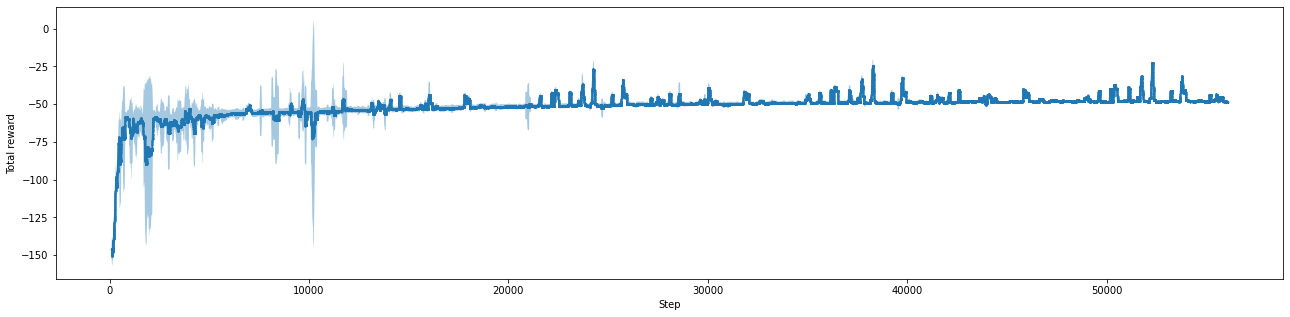
\includegraphics[width=.95\linewidth]{images/MVOberr/RL/RLrewards.png}
    \caption[Agent's rewards]{Agent's rewards over time. The reward is averaged over a rolling window of 96 time steps. The shadow region is $\pm2$ standard deviations calculated over 5 runs.}
    \label{im:4_rewards}
\end{figure}
\noindent From figure \ref{im:4_rewards}, it is possible to see that the agent is learning, since the total reward is increasing over time.\\

For all the 5 runs, after training, the agent was evaluated on the test set. Here reported are the results from one of the best run:
\begin{figure}[H]
\centering
    \subfloat[\label{fig:crit_sit_bef}]        {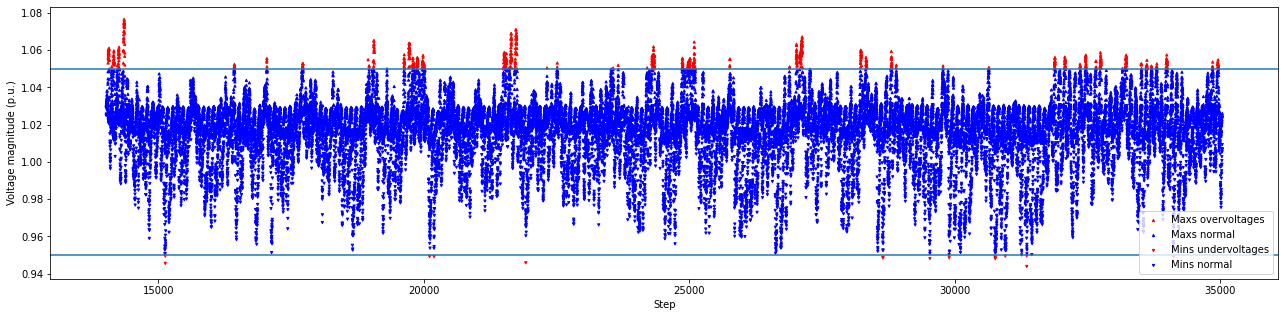
\includegraphics[width=0.85\linewidth]{images/MVOberr/CritialSituationsBefore.png}}\\
    
    \subfloat[\label{fig:crit_sit_aft}]       {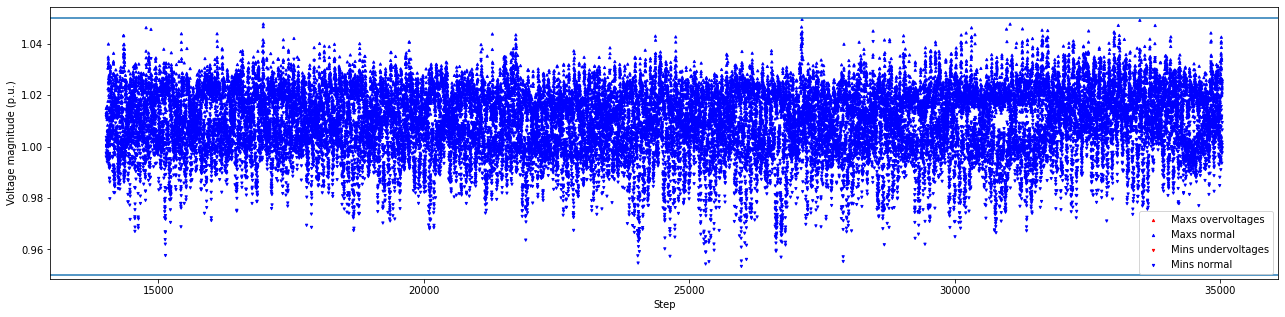
\includegraphics[width=0.85\linewidth]{images/MVOberr/RL/CritialSituationsAfter.png}}\\

    % 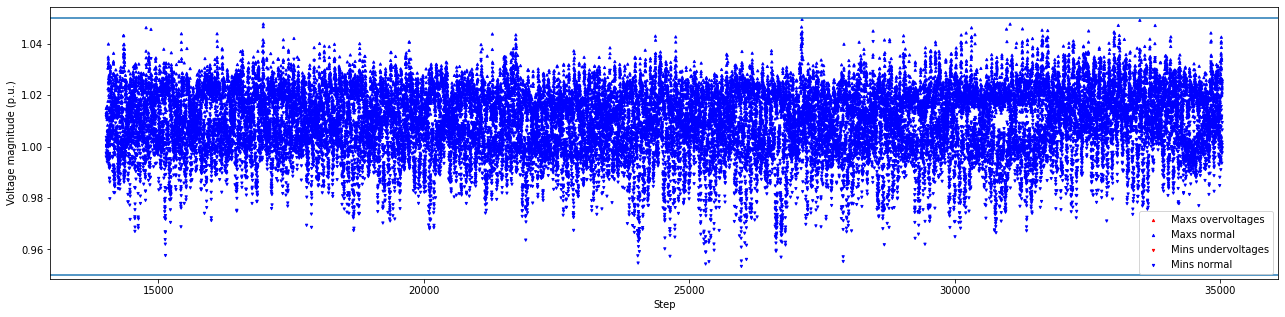
\includegraphics[width=0.9\linewidth]{images/MVOberr/RL/CritialSituationsAfter.png}
    \caption[Agent's solution to voltage problems]{The buses' voltage situation before (\textbf{a}) and after (\textbf{b}) the agent's actions.}
    \label{im:4_prosolv}
\end{figure}
\noindent Figure \ref{im:4_prosolv} shows that the agent was able to solve all the over voltage problems without introducing under voltages problems, that were solved as well.

\begin{algorithm}
    \STATE Total energy 169187 MW, total curtailed energy: 0.91 MW in 21024 time steps (7 months and 13 days), ratio: $5.3 \cdot 10^{-6}$ \%\\
    
    \STATE Total reactive power controlled: 287085 M\gls{VAR}
\end{algorithm}
\noindent the percentage of curtailed energy is well below the tolerable values of 4\%. Indeed, curtailment levels have generally been 4\% or less of wind energy generation in regions where curtailment has occurred \cite{enercurt}.\\
While the reactive power corresponds to an average of 0.22 M\gls{VAR} for device.\\

\noindent Some statistic from figure \ref{im:4_prosolv} are  reported here:

\begin{algorithm}[ht]
    \STATE Maximum voltage observed: 1.0494 \gls{pu} \\
    \STATE Minimum voltage observed: 0.9533 \gls{pu}
\end{algorithm}
\noindent So the agent understood how to control the network minimising the control needed, since the values are really close to the boundaries (1.05 \gls{pu} and 0.95 \gls{pu}) but inside the safe voltage condition.\\

In all the 5 runs the agent was able to solve the over voltage problems and in only one run some under voltages conditions were not solved.\\
It has also must be said that the agent performance is not perfect since the agent took some actions even it was not needed, it is also possible to see from figure \ref{im:4_rewards} is stuck in a local minimum, since the reward is steady around $-50$. \\

\noindent Here there are some more statistics for the best run:\\

\begin{algorithm}[h]
    \STATE Active power curtailment:\\
    \STATE needed (case 3: 1 - 0): 0.67 MW\\
    \STATE Not needed:\\
    \STATE case 1 (0 - 0): 0.24 MW\\
    \STATE case 2 (0 - 1): 0 MW\\
    \STATE case 4 (1 - 1): 0 MW\\
    
    \STATE Reactive power usage:\\
    \STATE needed (case 3: 1 - 0): 106341 MVAR\\
    \STATE Not needed:\\
    \STATE case 1 (0 - 0): 180744 MVAR\\
    \STATE case 2 (0 - 1): 0 MVAR\\
    \STATE case 4 (1 - 1): 0 MVAR
\label{alg:agentsucks}
\end{algorithm}
\noindent Cases, as defined in \ref{im:cases}, are reported here to check in which situation the agent decides to take a particular action.\\
In particular, the agent is able to understand when it is needed to perform the action (case 3) and in all those cases it can solve the voltage critical situation (case 4 situations are 0). Moreover, the agent newer worsened the situation of the network (case 2 situations are 0) but the agent could perform better since a lot of activity is done when not really needed (case 1).\\

The time for training the agent on average is 53 minutes and the inference time is 13 minutes.